Neutrino flavor oscillations are well established. This requires charged lepton flavor violation at some level as well.  However flavor violation in charged lepton interactions has never been observed.
If neutrino mass is the only source of new physics, and if
the mass generation occurs at a very high energy scale, CLFV processes are highly suppressed.  For example, if neutrinos are 
Dirac particles, the branching ratio for $\mu\rightarrow e\gamma$ is
\begin{equation}
BR(\mu \rightarrow e \gamma)=\frac{3\alpha}{32\pi}\left|\sum_i U_{\mu
i}^* U_{e i}\frac{m_{\nu_{i}}^2}{m_{W}^2}\right|^2 \sim 10^{-52}
\end{equation}
where $U_{ei}$ are the leptonic mixing matrix elements. This value,
which suffers from extreme suppression from the small neutrino masses,
is experimentally inaccessible. In many extensions of the Standard Model
however, there are much larger contributions to CLFV and current experimental bounds set strict limits on the parameter space available for new physics models.


The effective Lagrangian relevant for the $\mu \rightarrow e\gamma$ and $\mu^+ \rightarrow e^+e^-e^+$ decays can be parametrized,
regardless of the origin of CLFV, as
\begin{eqnarray}
{\cal L}_{\mu\rightarrow e\gamma, eee} &=& -{4G_{F}\over\sqrt{2}}
\left[  {m_{\mu }}{A_R}\overline{\mu_{R}}
        {{\sigma }^{\mu \nu}{e_L}{F_{\mu \nu}}}
       + {m_{\mu }}{A_L}\overline{\mu_{L}}
        {{\sigma }^{\mu \nu}{e_R}{F_{\mu \nu}}} \right. \nonumber \\
    && + {g_1}(\overline{{{\mu }_R}}{e_L})
              (\overline{{e_R}}{e_L})
       + {g_2}(\overline{{{\mu }_L}}{e_R})
              (\overline{{e_L}}{e_R}) \nonumber \\
    &&   +{g_3}(\overline{{{\mu }_R}}{{\gamma }^{\mu }}{e_R})
              (\overline{{e_R}}{{\gamma }_{\mu }}{e_R})
       + {g_4}(\overline{{{\mu }_L}}{{\gamma }^{\mu }}{e_L})
              (\overline{{e_L}}{{\gamma }_{\mu }}{e_L})  \nonumber \\
    && \left.  +{g_5}(\overline{{{\mu }_R}}{{\gamma }^{\mu }}{e_R})
              (\overline{{e_L}}{{\gamma }_{\mu }}{e_L})
       + {g_6}(\overline{{{\mu }_L}}{{\gamma }^{\mu }}{e_L})
              (\overline{{e_R}}{{\gamma }_{\mu }}{e_R})
       +  h.c. \right].
       \label{CL:int}
\end{eqnarray}
The decay $\mu \rightarrow e\gamma$ is mediated by the first two terms 
of Eq. (\ref{CL:int}), the dipole terms.  These
terms, as well as the remaining contact terms, all contribute to the 
decay $\mu^+ \rightarrow e^+e^-e^+$.  The relative strength of
these decay rates depends on the relative strength of the dipole and contact terms. 
 Turning this around, searches for
these two decays reveal much about the underlying flavor structure.  
In some models the dipole contribution 
dominates both decays.  In this case, a simple relation
exists for the relative branching ratio:
\begin{equation}
\frac{B(\mu^{+}\rightarrow e^{+}e^{-}e^{+})}{B(\mu^{+} \rightarrow
e^{+} \gamma)} \simeq
\frac{\alpha}{3\pi}\left(\ln(\frac{m_{\mu}^{2}}{m_{e}^{2}})-\frac{11}{4}\right)
= 0.006.
\label{CL:branching}
\end{equation}
However, contact terms arise
frequently in popular models where the relation
Eq. (\ref{CL:branching}) does not hold.  A good example is the type II seesaw mechanism for small neutrino masses.  Here, one
does not add right-handed neutrinos to the spectrum, rather one
includes an iso--triplet scalar $\Delta = (\Delta^{++},\,\Delta^+,\,\Delta^0)$ with quantum numbers
$(1,3,+2)$ under $SU(3)_c \times SU(2)_L \times U(1)_Y$.  Neutrino
masses are generated via the Yukawa coupling $\frac{f_{ij}}{2}
\ell_i^T C \ell_j \Delta$, once a nonzero $\langle
\Delta^0\rangle$ develops.  The doubly charged scalar
$\Delta^{++}$ could mediate the decay $\mu^+
\rightarrow e^+e^-e^+$ at tree level.  In this case, the branching ratios for $\mu
\rightarrow e\gamma$ and $\mu^+ \rightarrow e^+e^-e^+$ become comparable.

%\begin{figure}[t]
%\begin{center}
%\includegraphics[width=4cm]{mu_3e_doubly_charged.pdf} \hspace*{0.3in}
%\includegraphics[width=4.8cm]{mu_plus_e_minus.pdf}
%\caption{\label{CL:doubly}$\mu \rightarrow 3e$ decay (left) and muonium-antimuonium conversion (right)
%mediated by doubly charged scalar.}
%\end{center}
%\end{figure}

\begin{figure}[t]
\begin{center}
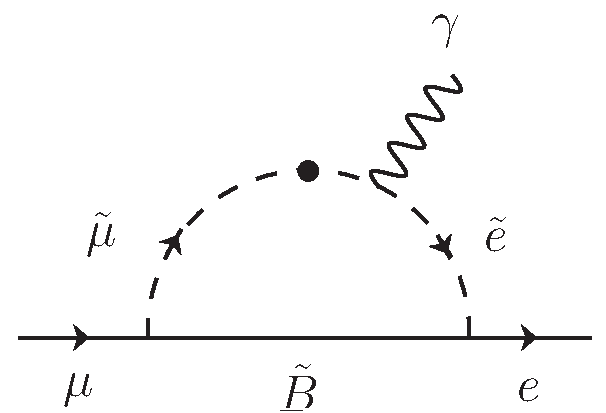
\includegraphics[width=5cm]{ChargedLeptons/Figures/mu_e_gamma.pdf} \hspace*{2cm}
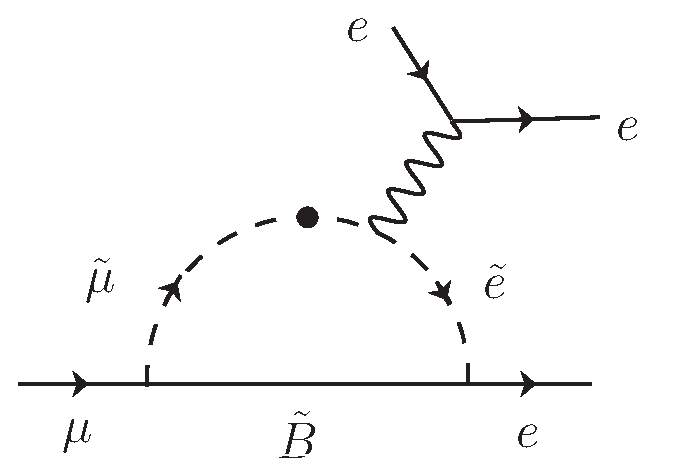
\includegraphics[width=5cm]{ChargedLeptons/Figures/mu_3e.pdf}
\caption{\label{CL:mutoegamma}$\mu \rightarrow e\gamma$ decay mediated by SUSY particles (left panel), and $\mu \rightarrow 3e$ decay (right panel).}
\end{center}
\end{figure}

Equally important as the decays $\mu \rightarrow e\gamma$ and $\mu^+
\rightarrow e^+e^-e^+$ is the coherent $\mu^-N \rightarrow e^-N$ conversion
process in nuclei.  Muonic atoms are formed
when negative muons are stopped in matter.  In the ground state of these
atoms, the muon can decay in orbit or be captured with the emission of
a neutrino via the process $\mu^{-} + (A,Z) \rightarrow
\nu_{\mu} + (A,Z-1)$.  If there are new sources of CLFV, muon capture
without the emission of a neutrino can occur: $\mu^{-} + (A,Z)
\rightarrow e^{-} + (A,Z)$.   This would occur in supersymmetry (SUSY)  via
the diagram of Fig.~\ref{CL:mutoegamma}, when the photon is attached to
a quark line.  Like $\mu^+\rightarrow e^+e^-e^+$, this process can occur through dipole
interactions or through contact interactions.  Such contact
interactions arise naturally in leptoquark models at the tree level,
while in  SUSY the dipole interactions dominate.  If only the
dipole couplings are important, one can obtain a relation for the ratio of rates
\begin{equation}
\frac{B(\mu^{+}\rightarrow e^{+}\gamma)}
{B(\mu^{-}N\rightarrow e^{-}N)}
=\frac{96\pi^{3} \alpha}{G_F^2 m_{\mu}^4}\cdot
{1\over{3\cdot 10^{12}B(A,Z)}}\simeq \frac{428}{B(A,Z)},
\end{equation}
where $B(A,Z)$ is a function of the atomic number and atomic weight,
with its value ranging from 1.1 to 2.2 for Al, Ti and Pb atoms.  
The best limits on these processes are $B(\mu^- + {\rm Ti}
\rightarrow e^- + {\rm Ti}) < 4.3 \times 10^{-12}$~\cite{Dohmen:1993mp} and $B(\mu^- + {\rm Au}
\rightarrow e^- + {\rm Au}) < 7.0 \times 10^{-13}$~\cite{Bertl:2006up} from experiments conducted at PSI.
For these searches the limits quoted are with respect to the muon capture process $\mu^{-} + (A,Z) \rightarrow \nu_{\mu} + (A,Z-1)$.
Future
experiments can improve tremendously on these limits down to  $10^{-18}$.

A related process is the incoherent, lepton number violating
process $\mu^{-} + (A,Z) \rightarrow e^{+} + (A,Z-2)^{*}$, which
occurs in left--right symmetric models via the exchange of
right--handed neutrinos and $W_R^\pm$ gauge bosons.  The best limit
presently on this process is $B(\mu^- + {\rm Ti} \rightarrow
e^+ + {\rm Ca}) < 1.7 \times 10^{-12}$, also from PSI.  TeV scale
left--right symmetry predicts observable rates for this
transition.

CLFV could also be seen in other muonic systems.  Muonium is a  ($\mu^+ e^-$) bound state   analogous to the hydrogen atom, which
in the presence of a CLFV interaction can oscillate into antimuonium
($\mu^-e^+$).  The doubly charged scalar of the seesaw model, the left--right
symmetric model, or the radiative neutrino mass model would all lead to
this process.  If
the Lagrangian for this process is parametrized as
\begin{equation}
H_{\rm Mu\overline{Mu}} = \left({G_{\rm Mu\overline{Mu}} \over
\sqrt{2}} \right)
\overline{\mu}\gamma_{\lambda}(1-\gamma_5){e}
\overline{\mu}\gamma^{\lambda}(1-\gamma_5){e} + h.c.,
\end{equation}
the current limit from PSI experiments is $G_{\rm Mu\overline{Mu}} < 0.003
\,G_F$, with room for improvement by several orders of magnitude in
the near future.



